\section{Optimal Control of Pitch/Travel without Feedback}\label{sec:prob2}

\begin{figure}[tp]
	\centering
		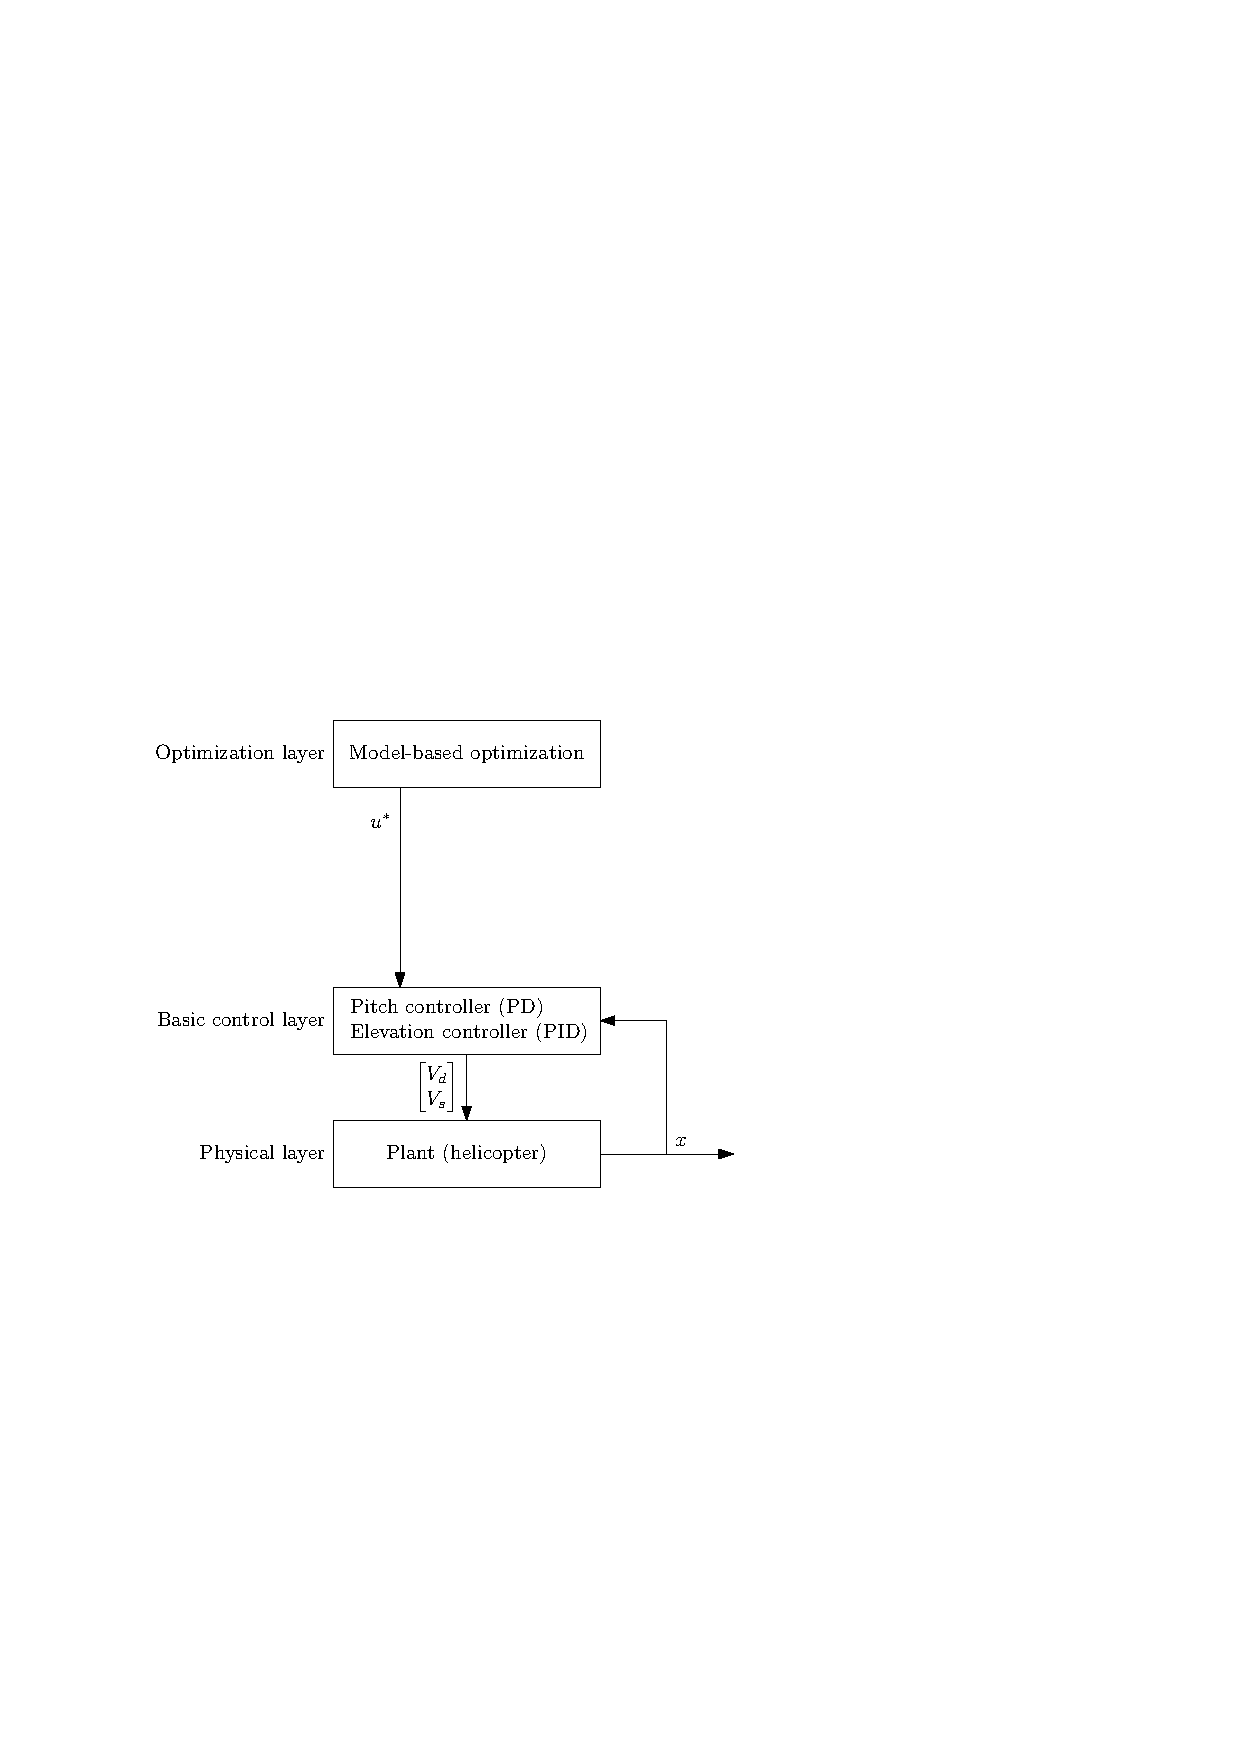
\includegraphics[width=1.00\textwidth]{figures/layers_openloop.pdf}
	\caption{A figure created with Ipe.}
	\label{fig:layers_openloop}
\end{figure}

\subsection{State space model}

\subsection{Discretization}

\subsection{Optimal trajectory}

Here is a matrix equation you can use as a template:
\begin{equation}
\begin{bmatrix}
 1 &  0 &  0 & 0 & -b &  0 &  0 &  0 \\
-a &  1 &  0 & 0 &  0 & -b &  0 &  0 \\
 0 & -a &  1 & 0 &  0 &  0 & -b &  0 \\
 0 &  0 & -a & 1 &  0 &  0 &  0 & -b                                
\end{bmatrix}
\begin{bmatrix} x_1 \\ x_2 \\ x_3 \\ x_4 \\ u_0 \\ u_1 \\ u_2 \\ u_3 \end{bmatrix}
=
\begin{bmatrix}
ax_0 \\ 0 \\ 0 \\ 0      
\end{bmatrix}
\end{equation}

\subsection{Results and discussion}

\begin{figure}[htb]
	\centering
		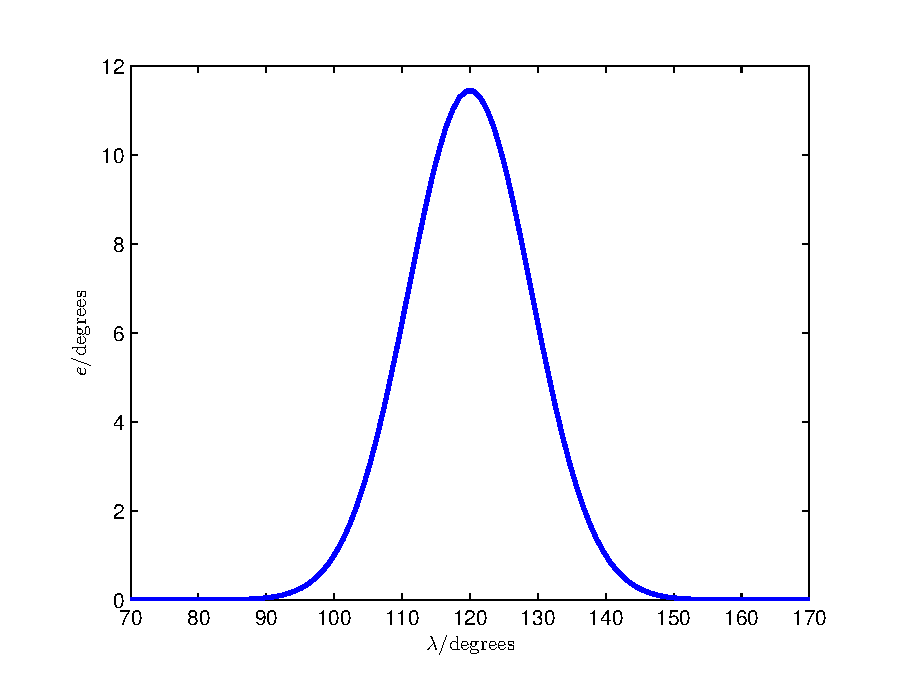
\includegraphics[width=0.8\textwidth]{figures/constraint_eps.eps}
	\caption{A plot in EPS format --- a much better idea.}
	\label{fig:constraint_eps}
\end{figure}
